\chapter{HDAC6 complex formation models robustly predict capsid breakage and in vivo responses to host pathway perturbations}
\label{ch:ReactionModels}

\dictum[Ann Leckie, "Ancillary Mercy"]{%
  "Why 1.11 meters? It doesn't seem like a terribly useful distance." \par
  "Well, no," replied Translator Zeiat, still frowning. "It wasn't meant to be a useful distance. In fact the distance wasn't meant at all... No, the bullets aren't designed to go through anything for 1.11 meters. They are designed to destroy Radchaai ships. That was what the purchasers required of them. The 1.11 meters is a kind of... accidental side effect sort of thing."}%
\vskip 1em

Parts of this chapter are to be submitted as: A. Artcibasova, L. Wang, S. Anchisi, Y. Yamauchi, M. Schmolke, P. Matthias, J. Stelling "A quantitative model for HDAC6-mediated virus uncoating predicts Influenza A infectivity"

\section{Introduction}

Using a biophysical model of capsid disassembly (Chapter \ref{ch:TugOfWar}) we were able to show that a tug-of-war mechanism of uncoating is feasible for certain combinations of molecular motors attached to the viral fusion pore. However, we do not know whether such motor recruitment is feasible \textit{in vivo}.

More generally, in part due to the difficulties of experimental measurements, there is no consistent understanding or quantitative description for any virus of how the various virus-host interactions integrate with the viral capsid mechanics to impact uncoating and ultimately infectivity. Here, we therefore combine computational modeling with experimental analysis insights to quantitatively elucidate the mechanisms of HDAC6-mediated uncoating of influenza A virus \textit{in vivo}. 

Previous studies highlighted the role of ubiquitin (Ub) in influenza uncoating \cite{rudnicka2016ubiquitin}: influenza virus carries high numbers of cellular Ub B \cite{hutchinson2014conserved}, itchy E3 ubiquitin protein ligase ubiquitinates M1 capsid protein, promoting influenza escape from late endosomes \cite{su2013pooled}, and the depletion of E3 ubiquitin ligase cullin 3 inhibits influenza uncoating \cite{hubner2012cullin, huotari2012cullin}. These results, coupled with the crucial role of HDAC6-ZnF during influenza uncoating \cite{banerjee2014influenza} suggest that Ub may serve as an interface between capsid protein M1 and HDAC6.

However, biochemical analysis by our collaborators from Patrick Matthias' group at FMI identified an essential role for unanchored ubiquitin chains in bridging HDAC6-myosin interaction. The sizes and geometries of HDAC6 and molecular motors render these two possibilities for HDAC6-Ub interactions mutually exclusive. Furthermore, viral Ub interfacing HDAC6-M1 binding would lead to competition between viral and cellular Ub. On the other hand, if Ub is involved in molecular motor recruitment instead, cellular Ub would assist the binding, and viral Ub would simply support it via co-localization.

Using those experimental insights we developed three detailed biochemical-biophysical model that use capsid breakage probabilities, determined by our Mass-Spring model (Chapter \ref{ch:TugOfWar}). We showed that a competitive model with viral Ub interfacing HDAC-M1 interaction was unable to recruit molecular motors for any combinations of parameters. Meanwhile, models with Ub assisting motor recruitment robustly predict IAV uncoating efficiency \textit{in vivo} in unperturbed infection as well as across various perturbed conditions.

Our collaborators from Mirco Schmolke's group at University of Geneva demonstrated that the infectivity difference between two clinical influenza strains (H1N1 and H3N2) depends on a single amino acid variation between their M1 proteins. We use our combined biochemical-biophysical models to estimate how this difference affects binding to HDAC6, HDAC6-dependent uncoating, and infectivity. The results are consistent between experiments and model predictions, further supporting our tug-of-war mechanism for influenza A uncoating.

\section{Results}

\subsection{HDAC6 complex formation models predict capsid breakage robustly}

We aimed to integrate the biochemical interaction mechanisms determined by our collaborators from Patrick Matthias' group at FMI with the mechanics of virus uncoating quantitatively, for example, to determine how many cellular motors per exposed capsid are feasible in vivo, and how their actions will translate to virus uncoating (and eventually, infectivity). Because it was not possible to define all interaction mechanisms unambiguously, we formulated three reaction model schemes for HDAC6 complex formation (Figure \ref{figure:ReactionModelSchemes}) that incorporate distinct mechanistic hypotheses (Figure \ref{figure:UbRoleHypotheses}). We based one model variant termed "Viral Ub" on the previously available uncoating data \cite{banerjee2014influenza}. It assumes competition between capsid-borne and cellular unanchored ubiquitin (Ub) chains for the zinc finger domain of HDAC6. The two model variants incorporating new biochemical protein interaction results assume that cellular ubiquitin chains either assist with binding of both myosin and dynein motors to HDAC6 (variant "Symmetric"), or only with binding of myosin (variant "Asymmetric"). To estimate corresponding virus capsid breakage we used averaged estimates for molecular motor complex recruitment (see Methods \ref{ch:ReactionModelsMethods}, Appendix \ref{appendix:reactionModelsEquations} for details) together with interpolated capsid breakage (Figure \ref{figure:MassSpringInterpolation}) based on mass-spring model predictions from Chapter \ref{ch:TugOfWar}.

\begin{figure}
\begin{center}
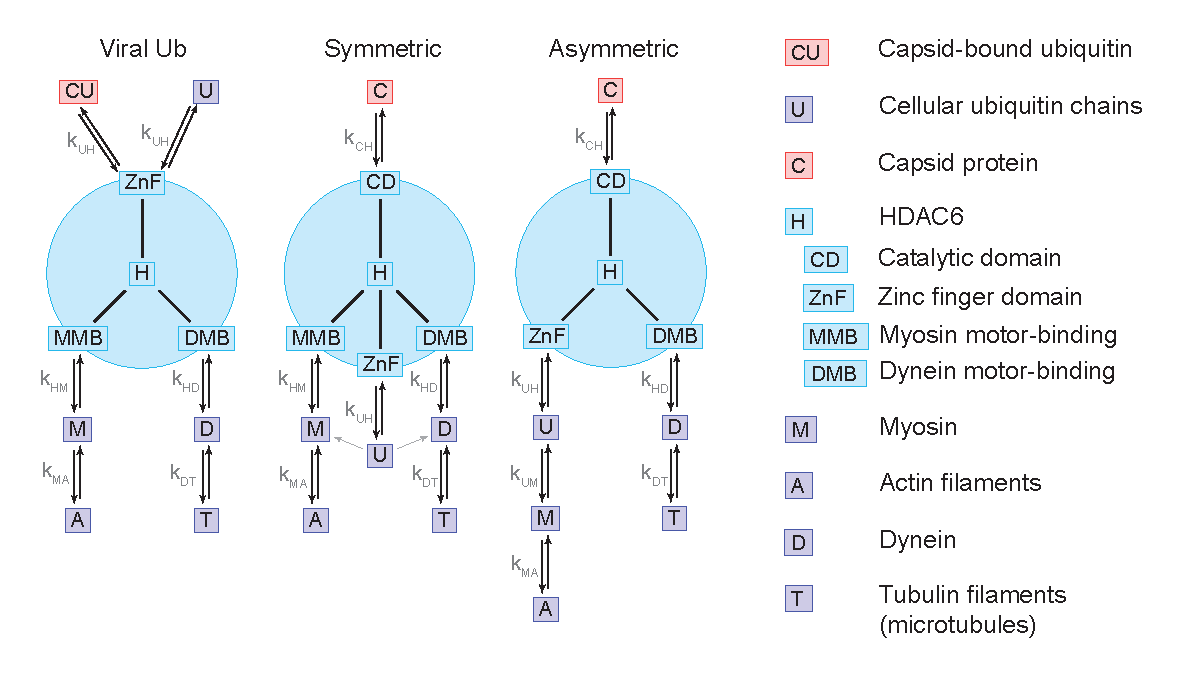
\includegraphics[width=0.95\textwidth, trim={0cm 0cm 0cm 0cm}, clip]{D_chapters/2_ReactionModel/ReactionModels.pdf}
\caption[Interaction schematics for the three reaction model variants]%
{Interaction schematics for the three reaction model variants. Nodes represent proteins or protein domains (linked by solid lines) and arrows denote biochemical reactions with their corresponding on-rates indicated next to the arrows. Node colors distinguish between viral proteins (red), HDAC6 (cyan), and other host proteins (purple).}
\label{figure:ReactionModelSchemes}
\end{center}
\end{figure}

To make the models consistent with prior \textit{in vivo} data, we used published reaction rate parameters for proteins of interest (or averages and similar parameters where data was not available) as well as protein abundances in lung tissues from proteomicsDB \cite{schmidt2018proteomicsdb}. Even when we widely sampled the reaction rate parameters uniformly (with fixed protein concentrations), the "Viral Ub" model failed to generate capsid breakage for any combination of reaction rate parameters. We then optimized unknown and imprecise reaction rate parameters for the other two models to achieve both myosin and dynein recruitment, and thereby maximize breakage, while keeping the reaction rate parameters close to literature values. This yielded reference parameter sets for each model variant. To represent the model uncertainty and to assess its effect on model predictions, we then sampled total protein concentrations normally around the means of previously reported values, and rate parameters log-normally close to their reference values (see Methods for details).

We used the reaction model to compute motor complex abundances for the "Symmetric" and "Asymmetric" model variants at steady state. Both variants can lead to motor complex configurations that are conducive to efficient virus uncoating (see Figure \ref{figure:densitiesRCsupplementary}), but the "Asymmetric" variant leads to higher myosin and dynein binding (Figure \ref{figure:densitiesRC}). Next, we used the mass-spring mechanical model to predict average capsid breakage probabilities from the motor configurations (see Methods). The "Asymmetric" model variant showed a higher density of capsid breakage probabilities close to 100\% for uniform sampling (Figure \ref{figure:densitiesRC} (uniform)), indicating efficient virus uncoating. We obtained qualitatively similar results with a different sampling strategy (Figure \ref{figure:densitiesRC} (normal)). Thus, our models – which incorporate both known constraints and uncertainties – suggest that ubiquitin chains are important for forming motor complexes and thereby for efficient capsid breakage.

\begin{figure}
\begin{center}
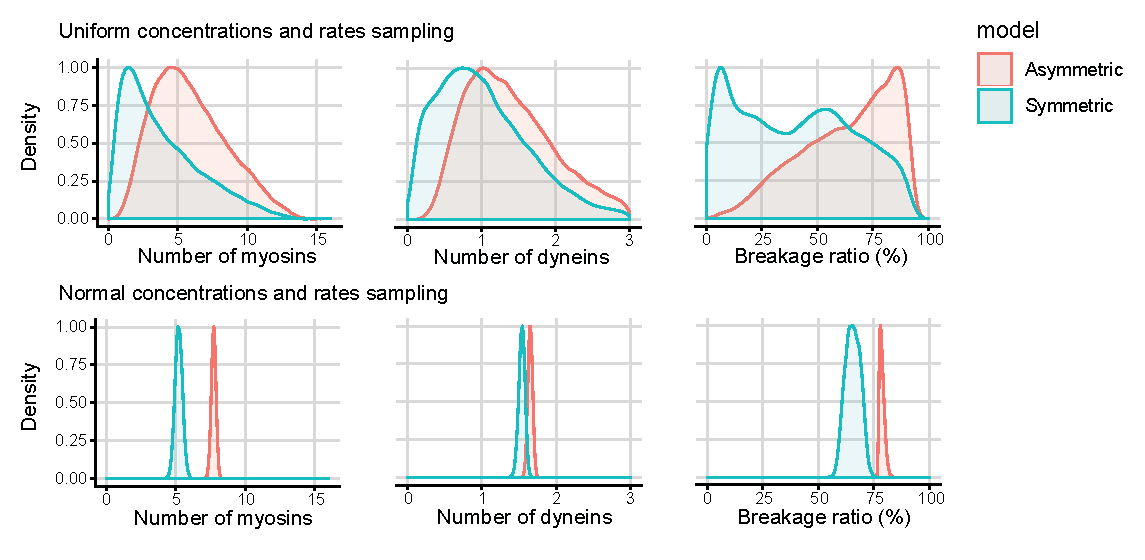
\includegraphics[width=0.95\textwidth, trim={0cm 0cm 0cm 0cm}, clip]{D_chapters/2_ReactionModel/densitiesRC.pdf}
\caption[Molecular motor and capsid breakage density distributions based on joined sampling of rates and concentrations]%
{Density distributions of number of myosin motors (left), number of dynein motors (middle), and capsid breakage probabilities (right) for the "Symmetric" and "Asymmetric" reaction model variants. Initial concentrations and reaction rate constants were sampled uniformly or normally around literature values and rate constant values were adjusted accordingly. The "Asymmetric" model variant allows for relatively high amounts of myosins and dyneins, and total highest breakage probability (see Methods for details). All the densities were normalized by their peak for easier comparison.}
\label{figure:densitiesRC}
\end{center}
\end{figure}

\begin{figure}
\begin{center}
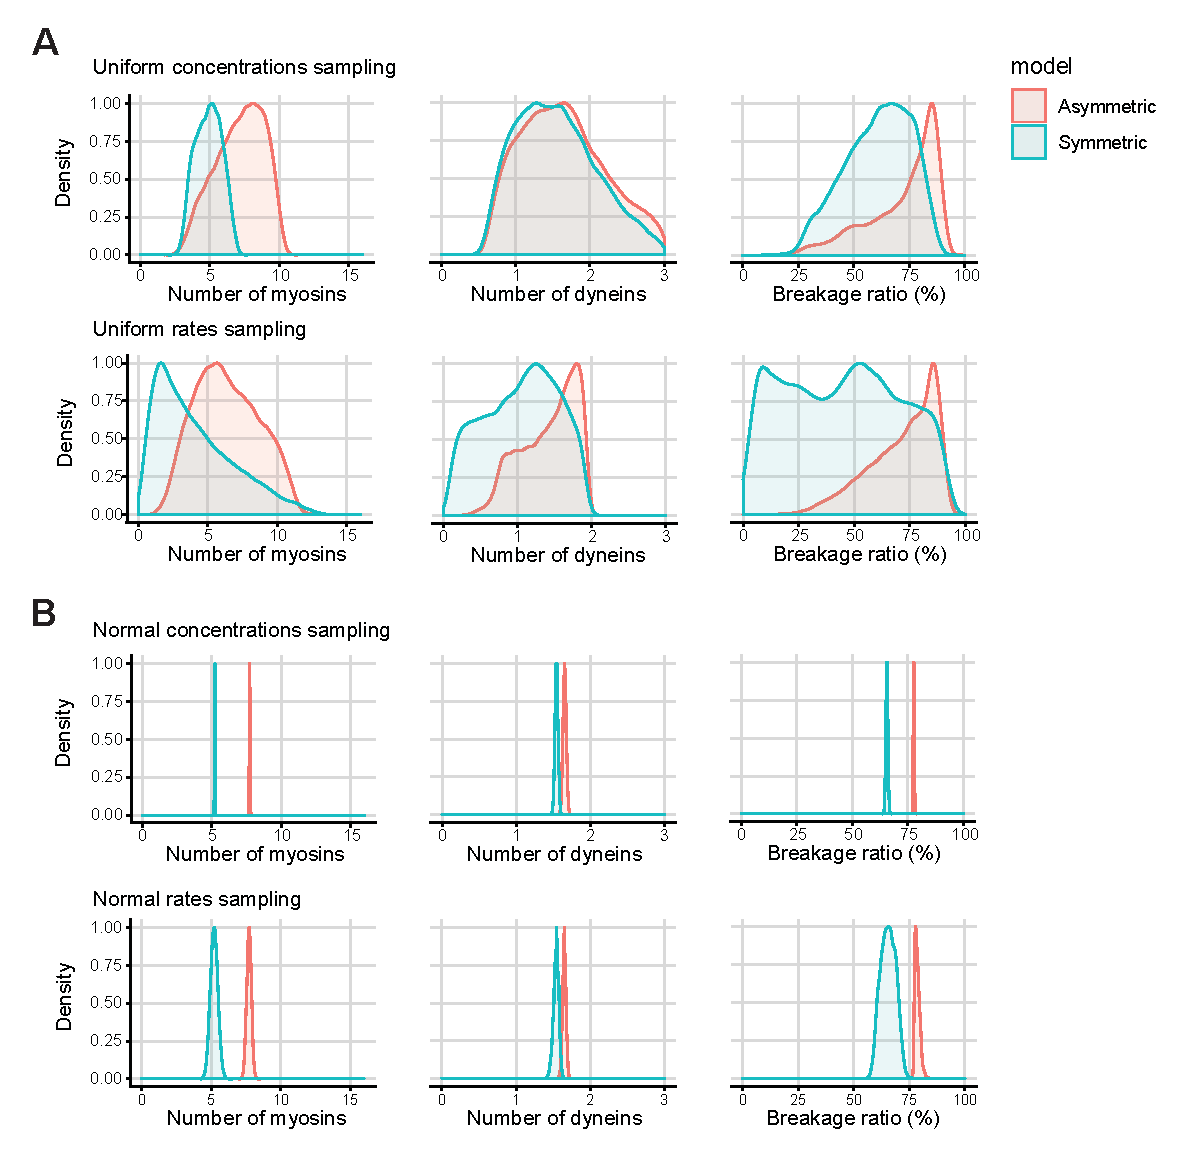
\includegraphics[width=0.95\textwidth, trim={0cm 0cm 0cm 0cm}, clip]{D_chapters/2_ReactionModel/densitiesRCsupplementary.pdf}
\caption[Molecular motor and capsid breakage density distributions based on joined sampling of rates or concentrations]%
{Reaction models' density profiles for the numbers of myosin and dynein motors and for the estimated capsid breakage ratio for (A) uniformly or (B) normally jointly sampled rates or concentrations. All the densities were normalized by their peak for easier comparison.}
\label{figure:densitiesRCsupplementary}
\end{center}
\end{figure}

To identify critical factors for efficient virus uncoating, we varied individual total protein concentrations and rate parameters (Figure 4C, D). Both model variants showed similar sensitivities in the examined ranges. The capsid breakage probability was not sensitive to changes of capsid protein M1 abundance (due to averaging by the number of virions). A decrease in tubulin concentrations led to a weak increase in capsid breakage. In contrast, we observed a peak close to the reference point for dynein, myosin, and HDAC6 concentrations, suggesting an optimal abundance of these proteins for uncoating. For the "Asymmetric" model, changes in ubiquitin elicited a similar peak-like shape, while for the "Symmetric" variant, we observed a plateau. This trend is reversed for the model variants’ actin dependencies. For most of the on-rates, capsid breakage is largely insensitive to changes of reaction rate parameters. However, the "Asymmetric" model is not sensitive to changes in  $k_{CH}$, but sensitive to low values of $k_{UH}$. The reverse holds for the "Symmetric" model. Dissociation constants did not affect capsid breakage at low values, then, sometimes, reached a small peak, and dropped dramatically. One notable difference between the models is that in the "Asymmetric" ("Symmetric") case, $K_{UH}$ ($K_{HM}$) peaks near the reference point, which can be explained by those two reaction rates controlling HDAC6-myosin binding, respectively. Overall, we conclude that our models that combine the biochemistry and mechanics of HDAC6-mediated uncoating can yield robust predictions of capsid breakage \textit{in vivo}, based on the identified mechanism with asymmetric influence of Ub chains on motor binding.

\subsection{The models predict in vivo responses to host pathway perturbations}

To assess to what extent the model predictions match with independent experimental observations \textit{in vivo}, namely previously published virus uncoating data \cite{banerjee2014influenza}, we first analyzed how uncoating efficiency is affected by perturbations in components of the host cell. We generated predictions with both model variants after introducing model perturbations that correspond to, or are at least similar to, the experimental perturbations (see Methods and Table S3). Specifically, most of the proposed perturbations are relatively straightforward to incorporate, by assuming a reduction of available reactants. For CiliobrevinD, we assume that immobile dyneins do not contribute to capsid breakage (technically it is possible that these fixed motors exert force by holding the capsid protein matrix in place). We represent protein domain mutations – HDAC6 $\Delta$DMC MEF cell line and HDAC6 ZnFm (W1116A) MEF cell line – through increased dissociation constants between HDAC6 and dynein ($K_{HM}$) or ubiquitin ($K_{UH}$), motivated by the model being sensitive to changes in these parameters (Figure \ref{figure:sampledTrajectories}).

\begin{figure}
\begin{center}
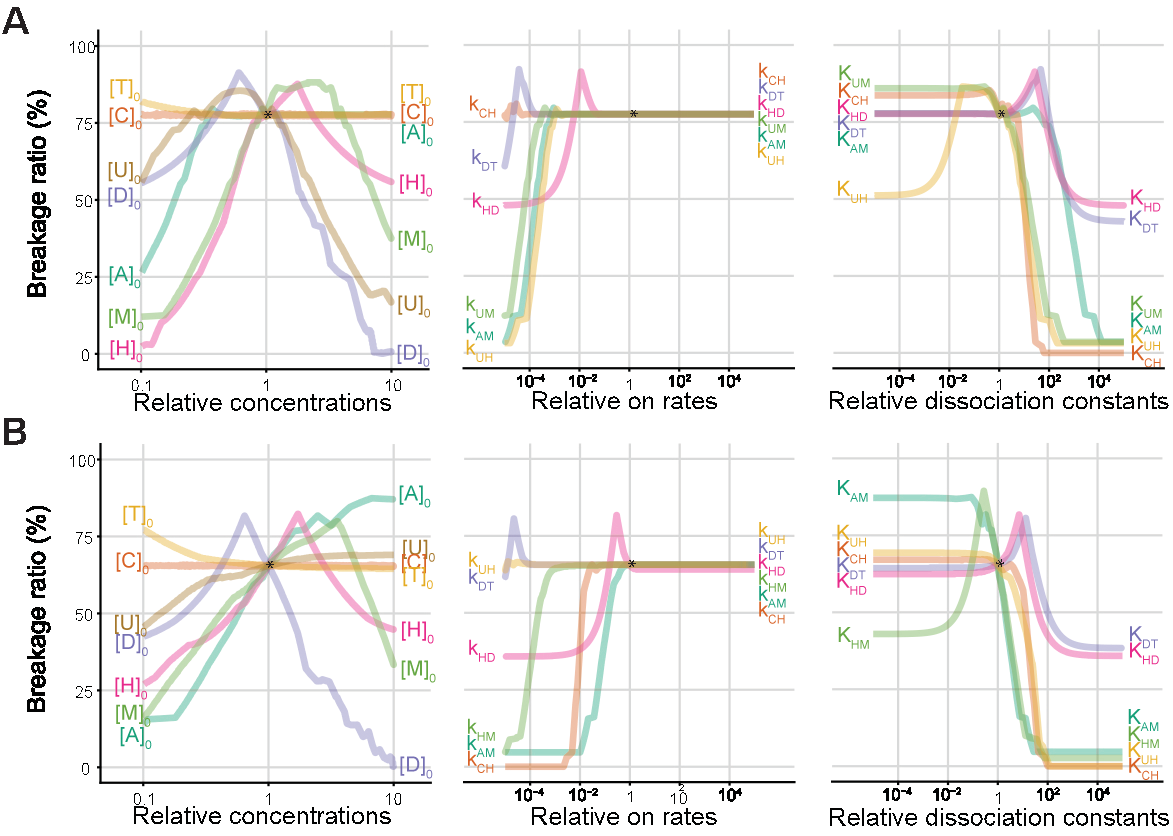
\includegraphics[width=0.95\textwidth, trim={0cm 0cm 0cm 0cm}, clip]{D_chapters/2_ReactionModel/SampledTrajectories.pdf}
\caption[Influence of varying individual initial protein abundances and reaction rate parameters on the capsid breakage probability]%
{Influence of varying individual initial protein abundances and reaction rate parameters on the capsid breakage probability for the "Asymmetric" (A) and "Symmetric" (B) model. All the varied parameters were normalized by the values corresponding to the reference conditions.}
\label{figure:sampledTrajectories}
\end{center}
\end{figure}

First, we focused on perturbations of the host cell’s molecular motors. Experimental data on virus uncoating efficiency were obtained in acid bypass assays that mimic normal infection by lowering the extracellular pH and blocking the natural acidification in endosomes \cite{banerjee2014influenza}. For the examined perturbations, the predicted median uncoating efficiencies agree well with the experimental results (Figure \ref{figure:reactionModelPredictions}A). The "Symmetric" predictions were slightly closer to the experimental results.

\begin{figure}
\begin{center}
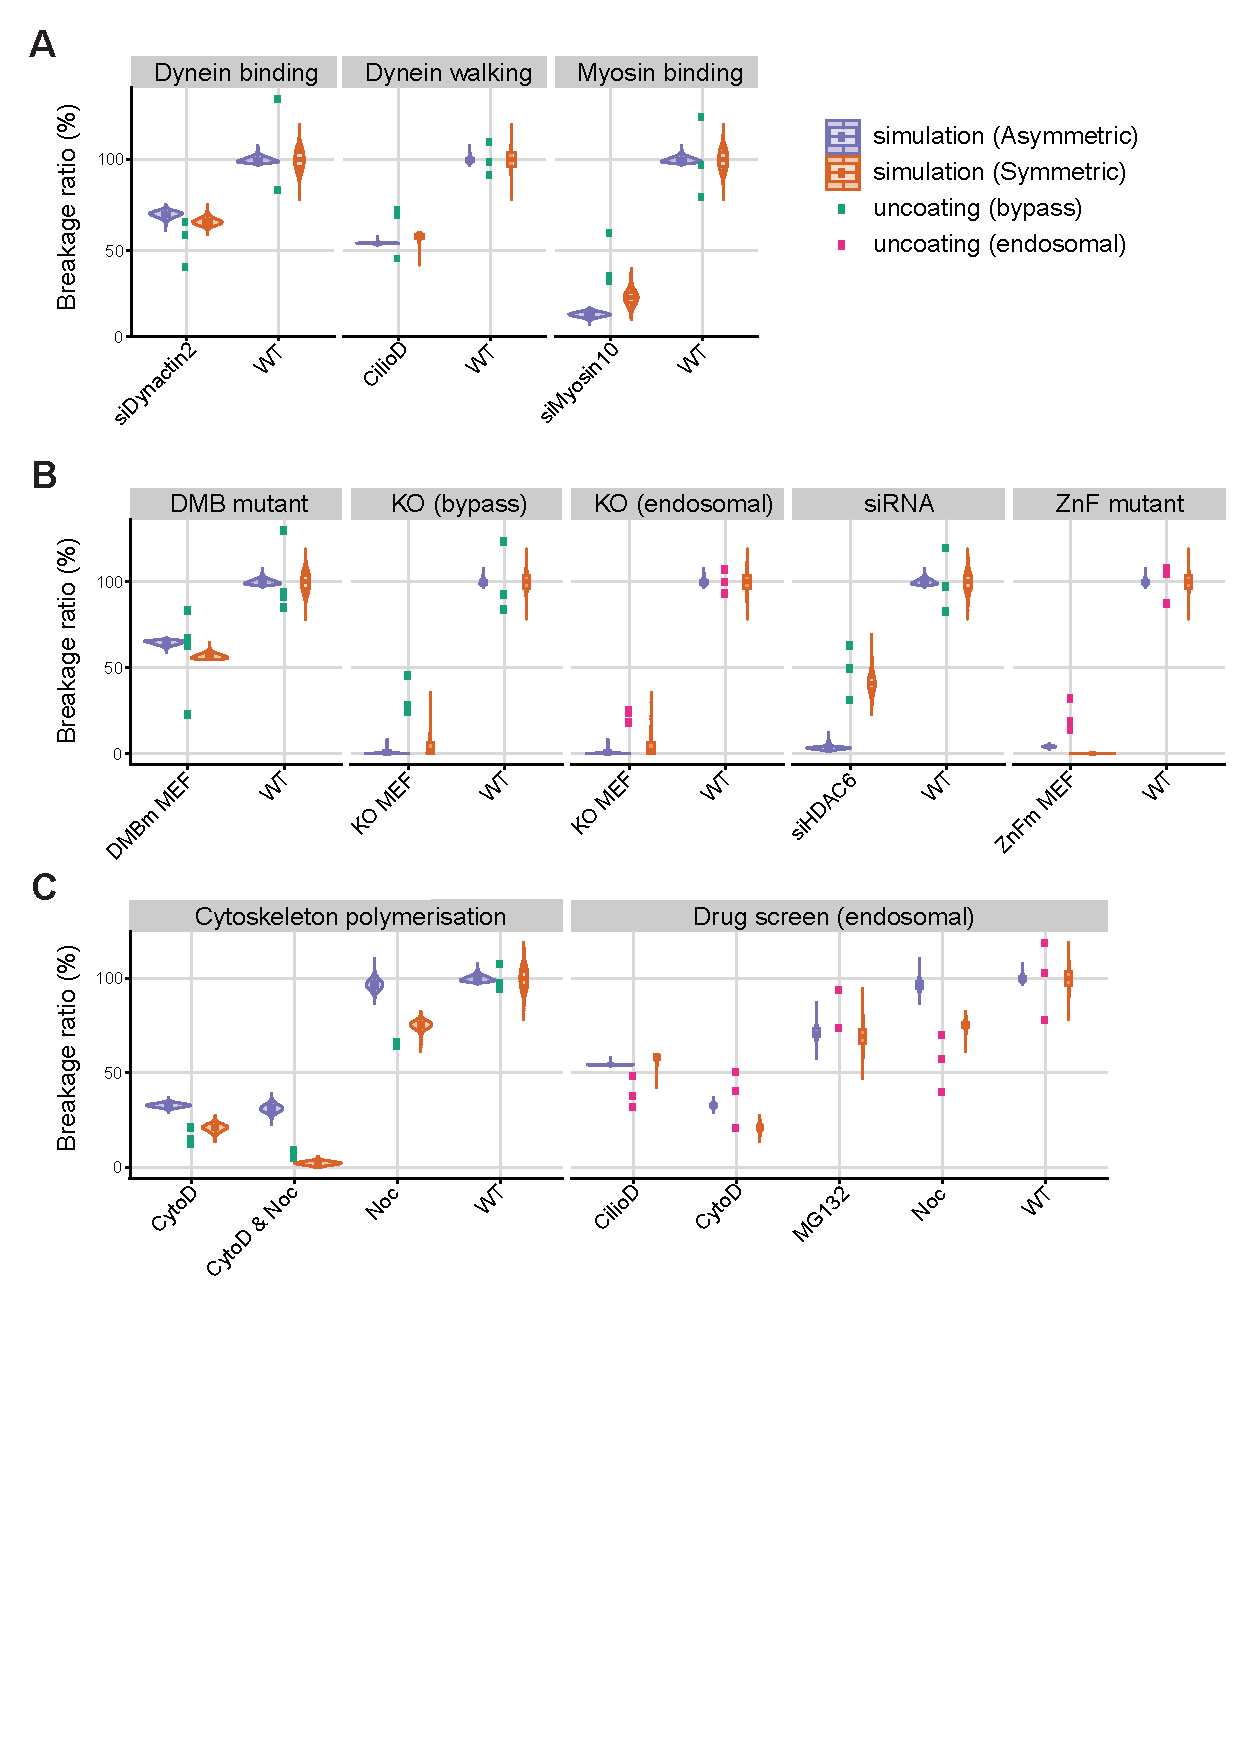
\includegraphics[width=0.8\textwidth, trim={0cm 8.5cm 0cm 0cm}, clip]{D_chapters/2_ReactionModel/FIGURE5_upd2.pdf}
\caption[The model predicts \textit{in vivo} uncoating efficiencies upon perturbations of the host cell]%
{The model predicts \textit{in vivo} uncoating efficiencies upon perturbations of the host cell.\par
Grey labels indicate the type of perturbations, and axis labels the specific experimental conditions.\par
(A) Perturbations of molecular motors.  Abbreviations: WT, wild type; siDynactin2, siRNA for Dynactin2; CilioD, Ciliobrevin D; siMyosin10, siRNA for myosin10. \par
(B) Perturbations of HDAC6. Abbreviations: DMBm, dynein motor binding mutant; KO, knock out; MEF, mouse embryonic fibroblasts; siHDAC6, siRNA for HDAC6; ZnFm, zinc finger mutant.\par
(C) Cytoskeletal perturbations and drug screen for inhibition of endosomal entry. Abbreviations: CytoD, Cytochalasin D; Noc, Nocodazole; CilioD, Ciliobrevin D.\par
All data shown are bypass (emerald) and endosomal (pink) experimental uncoating efficiencies and capsid breakage probabilities predicted by simulation of the "Asymmetric" (purple) and "Symmetric" (orange) reaction model with correspondingly perturbed initial conditions and rate parameters (see Methods \ref{ch:ReactionModelsMethods} for details). Experimental data are from \cite{banerjee2014influenza}. All data are normalized with respect to the untreated WT.
}
\label{figure:reactionModelPredictions}
\end{center}
\end{figure}

For a wide variety of HDAC6 perturbations, including knockdowns and mutations of specific domains, the models’ predictions aligned well with the experimental data (Figure \ref{figure:reactionModelPredictions}B). Notably, predictions were consistent with data from bypass experiments as well as experiments that measured endosomal uncoating in the normal virus infection pathway. Note, however, the difference in predicted viral capsid breakage probability in HDAC6 mutants or siRNA knockdown; the model only represents HDAC6-mediated uncoating, while \textit{in vivo} there are likely additional pathways or mediators capable of assisting in the uncoating \cite{gschweitl2016spopl,huotari2012cullin,miyake2019influenza,su2013pooled,yanguez2018phosphoproteomic}. The "Symmetric" model captured siRNA perturbations better than the "Asymmetric" variant, due to the former being less sensitive to reduction in HDAC6 (Figure \ref{figure:sampledTrajectories}), but the "Asymmetric" prediction for the ZnF mutant was closer to the experimental observation.

We compared model predictions with experimental data from perturbations of the host cell’s cytoskeleton and from an endosomal drug screen \cite{banerjee2014influenza} (Figure \ref{figure:reactionModelPredictions}C). Both variants performed well, with one notable exception: the "Asymmetric" variant did not capture the effect of nocadazole treatment, which is consistent with it being less sensitive to reduction in tubulin concentrations (Figure \ref{figure:sampledTrajectories}). Interestingly, except for nocodazole treatment, the "Asymmetric" variant performed better for endosomal perturbations (Figure \ref{figure:reactionModelPredictions}C, drug screen). Overall, we conclude that the combined model predictions compare well against published experimental data. Even when model limitations make the predictions imprecise, the models at the very least predict the correct direction of the perturbation effect on the viral capsid breakage probability. 

\subsection{Modelling HDAC6 inhibition dependency on M1}

Our collaborators from Mirco Schmolke's group at University of Geneva compared early replication efficacy of a panel of influenza A virus strains in wild type (WT) and HDAC6-deficient A549 lung epithelial cells (Figure \ref{figure:infectivityStrainSpecific}A). Strikingly, a clinical H3N2 isolate from 2013 displayed low dependence on HDAC6 for early replication steps as determined by automated fluorescence microscopy for viral nucleoprotein (NP). Specifically, this H3N2 isolate did not rely on a functional ZnF domain of HDAC6 while a clinical H1N1 isolate (pH1N1) from 2010 did. Inactivating HDAC6 deacetylase activity by a mutation in CD2 affected neither of the isolates (Figure \ref{figure:infectivityStrainSpecific}A). Sequence alignment of M1 from HDAC6-dependent (H1N1) and -independent (H3N2) viral strains revealed a single amino acid substitution (A218T in H3N2) (Figure \ref{figure:infectivityStrainSpecific}B) previously associated with matrix shape \cite{elleman2004m1}. Reversion of the 2003 H3N2 virus (A/Wyoming/03/2003) M1 residue 218 to alanine by reverse genetics restored HDAC6 dependence to a similar extent to H1N1 virus (Figure \ref{figure:infectivityStrainSpecific}A) and reduced particle length (not shown).

\begin{figure}
\begin{center}
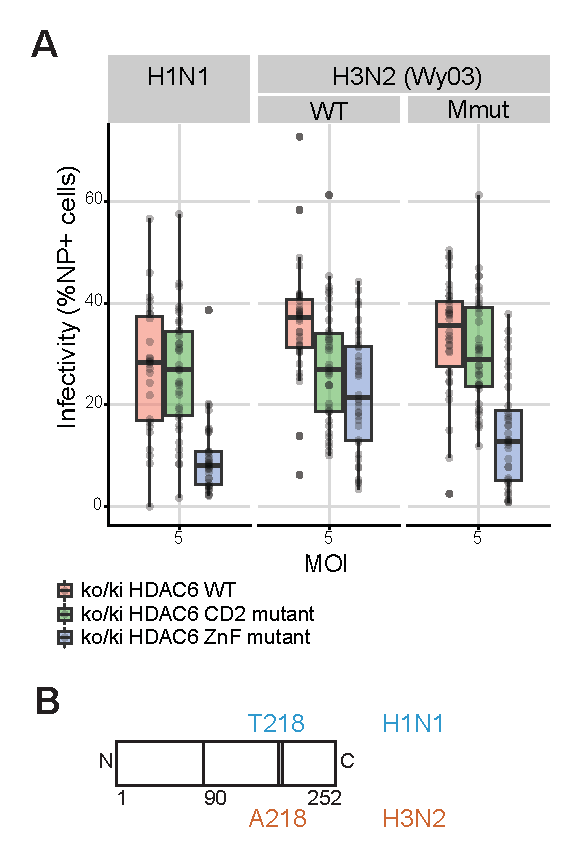
\includegraphics[width=0.7\textwidth, trim={0cm 0cm 0cm 0cm}, clip]{D_chapters/2_ReactionModel/FIGURE6_upd_infectivityStrainSpecific.pdf}
\caption[Influenza H1N1 shows stronger dependence on the HDAC6/aggresome pathway than H3N2]%
{(A) Influenza H1N1 shows stronger dependence on the HDAC6/aggresome pathway than H3N2. 
A549 cells expressing different HDAC6 versions (WT, CD2 mutant or ZnF mutant) were infected with pH1N1 or H3N2 virus at indicated multiplicity of infection (MOI) and cells were stained for viral NP. \par
(B) Schematic of H1N1 vs H3N2 M1 protein, highlighting residue 218. N and C denote N- and C-terminus. Numbers denote amino acid residues.}
\label{figure:infectivityStrainSpecific}
\end{center}
\end{figure}

Our collaborators from Patrick Matthias' group at FMI demonstrated that efficient co-immunoprecipitation of purified C-terminal M1 proteins with HDAC6 depends on alanine at position 218 of M1 (Figure \ref{figure:interactionM1ResidueSpecific}). Specifically, their data suggest that the A218T mutation reduces binding of M1 to HDAC6 by approximately two-fold (Figure \ref{figure:M1ReactionModel}).


\begin{figure}
\begin{center}
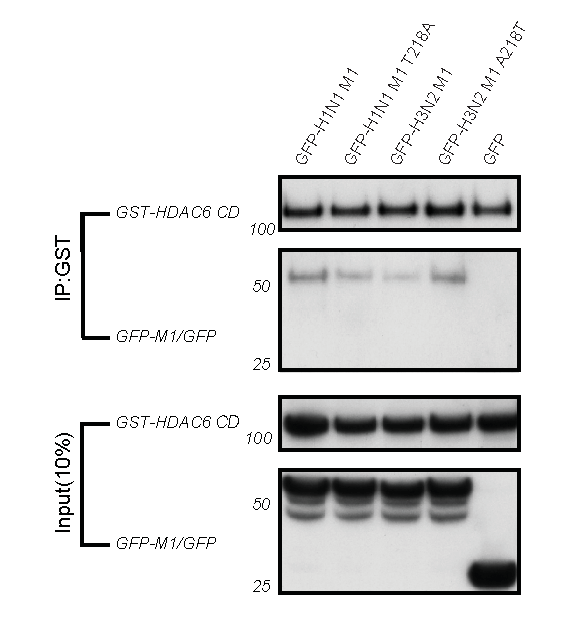
\includegraphics[width=0.8\textwidth, trim={0cm 0cm 0cm 0cm}, clip]{D_chapters/2_ReactionModel/FIGURE6_upd_IP.pdf}
\caption[Preferential interaction of viral H1N1 M1 protein with HDAC6 depends on residue T218.]%
{Preferential interaction of viral H1N1 M1 protein with HDAC6 depends on residue T218.\par
GFP-M1 fusion proteins (H1N1 WT or T218A, H3N2 WT or A218T) were transiently expressed in 293T cells and lysates were incubated with purified GST-HDAC6 (amino acids 82-837, catalytic domains) protein. GST-Trap beads were used to capture HDAC6 and associated proteins. The presence of diverse proteins in the precipitate (IP) or in the input lysate was determined by immunoblotting with anti-GFP (M1) or anti-GST (HDAC6) antibodies.}
\label{figure:interactionM1ResidueSpecific}
\end{center}
\end{figure}

To represent the effect of the amino acid substitution in the reaction models, we assumed that the M1 protein mutation affects the binding between the capsid and HDAC6, specifically the dissociation constant $K_{CH}$. We generated reaction model predictions for the mutant by choosing a multiplication coefficient for both models, setting the desired level of capsid breakage in an individual perturbation experiment (Figure \ref{figure:sampledTrajectories}) to the observed average level of M1 binding (Figure \ref{figure:interactionM1ResidueSpecific}). These model predictions aligned well with the experimental results from \textit{in vitro} M1 pull-down quantification and from in vivo automated fluorescence microscopy for both viral strains and their respective M1 mutants (Figure \ref{figure:M1ReactionModel}). However, the models did not fully capture interactions between different perturbations. For example, the relative infectivity of the pandemic H1N1 (pH1N1) strain in the HDAC6 ko/ki ZnF mutant cells corresponds to a reduction of the binding rate  between the HDAC6 ZnF domain and ubiquitin, and the infectivity of the H3N2 strain in HDAC6 ko/ki WT cells to the increased dissociation rate. Both cases lead to a reduction in capsid breakage. However, our NP fluorescence microscopy data for the H3N2 ko/ki ZnF mutant show a slight increase of viral entry compared to the ko/ki ZnF mutant (Figure \ref{figure:M1ReactionModel}), in contrast to either of the models. To summarize, these results suggest that the models represent key mechanisms of virus uncoating in vivo, despite focusing on only a few biochemical and mechanical interactions between virus and host components.

\begin{figure}
\begin{center}
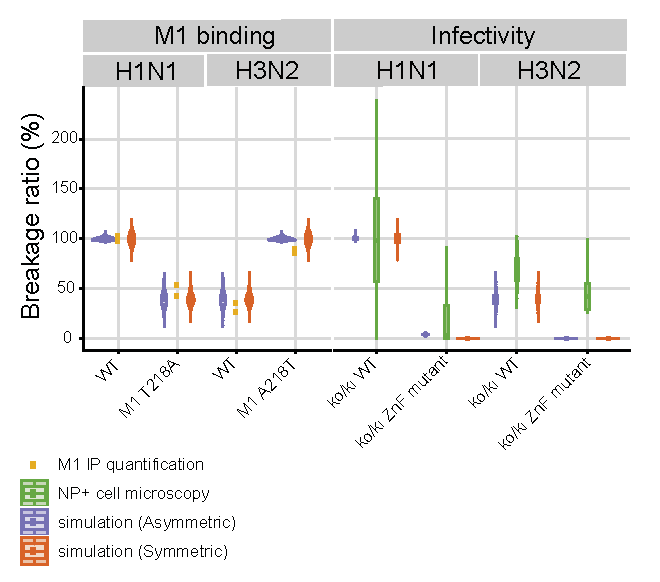
\includegraphics[width=0.8\textwidth, trim={0cm 0cm 0cm 0cm}, clip]{D_chapters/2_ReactionModel/FIGURE6_upd_simulation.pdf}
\caption[The model predictions for uncoating efficiencies based on strength of interaction between influenza M1 and HDAC6]%
{The model predictions for uncoating efficiencies based on strength of interaction between influenza M1 and HDAC6.\par
Experimental M1 IP quantification data from (C, yellow) and NP+ cell microscopy from (B, green) viral activities for perturbations of viral protein M1 variant for H1N1 and H3N2 viruses, compared against capsid breakage probabilities predicted by simulation of the "Asymmetric" (purple) and "Symmetric" (orange) reaction model with correspondingly perturbed initial conditions and rate parameters (see Methods for details). Abbreviations: IP, immunoprecipitation; NP+, nucleoprotein positive; ko/ki, knock out/knock in; WT, wild type; ZnF, zinc finger.
}
\label{figure:M1ReactionModel}
\end{center}
\end{figure}

\section{Discussion}

\subsection{A physically realistic tug-of-war model for IAV uncoating}

Uncoating is arguably an enigmatic step of virus entry, with only few detailed studies available for a limited set of viruses \cite{helenius2018virus, walsh2019exploitation}. As a transient step, uncoating is hard to measure quantitatively; for example, only recently have dynamic measurements in cells with complete influenza A viruses become possible using monoclonal antibodies \cite{banerjee2014influenza} or quantum dots \cite{qin2019real}. In addition, uncoating involves diverse (host and virus) components and interrelated (biophysical, biochemical, and cell biological) processes, making it difficult to integrate the relevant data and knowledge. These aspects may have contributed to limited conclusive evidence for a tug-of-war mechanism that has been proposed for several viruses \cite{banerjee2014influenza, lukic2014hiv, radtke2010plus, strunze2011kinesin}. However, the combination of biochemical analysis (Chapter \ref{ch:TugOfWar}) and mechanistic mathematical modeling (Chapter \ref{ch:ReactionModels}) described here for IAV uncoating demonstrates the feasibility of such integration, up to consistent predictions of differential infectivity of IAV strains with a single amino acid substitution in the M1 capsid protein.

Intriguingly, the model neither relies on exact knowledge of component concentrations and interaction parameters, nor on their direct estimation from experimental data except for M1 binding mutants, which could prevent truly independent predictions. We represented uncertainties explicitly, allowing us to integrate in a consistent manner relatively precise knowledge such as molecular motor forces with much less certain aspects such as binding affinities to make the model physically realistic. Despite these uncertainties being reflected in model predictions, the qualitative and often quantitative agreement with the experimental data indicates substantial robustness to assumptions made in model construction. In general, we aimed to identify core mechanisms that suffice to explain the collected experimental observations on IAV uncoating using a minimal model. We assume, for example, singular bonds between M1s in the capsid, no influence of endosomal transport on the tug-of-war mechanisms, and maximal capsid breakage for reaction rate optimization. This minimal nature of the model also implies that pleiotropic effects of perturbations are not well captured. For example, discrepancies for nocadazole experiments may arise because the drug not only disrupts microtubule dynamics, but also affects cell metabolism and viral traffic \cite{naghavi2017microtubule}.

\subsection{Mechanisms of IAV uncoating}

For a mechanistic interpretation, it is important that our model does not represent directional transport by multiple motors associated to a cargo \cite{hancock2014bidirectional}, but rather the generation of mechanical forces by the molecular motors. The high consistency between our model predictions and experimental data, however, argues against a mere positioning effect of the capsid inside the cell as a condition for uncoating, as hypothesized in early tug-of-war concepts \cite{lukic2014hiv, radtke2010plus}. The recent discovery of two host proteins activated early in infection and facilitating IAV uncoating supports this notion. Epidermal growth factor receptor pathway substrate 8 (EPS8) possibly fulfills a function in uncoating by modulating actin dynamics \cite{larson2019eps8}. G protein-coupled receptor kinase 2 (GRK2) appears to act via non-canonical targets \cite{yanguez2018phosphoproteomic}, and it is known to control cytoskeletal dynamics as well.

In more detail, a key element of our proposed mechanism is the ubiquitin-mediated binding between HDAC6 and molecular motors. Future studies should identify the source and nature of the binding-mediating ubiquitin chains. They could be provided by the virus \cite{banerjee2014influenza}, or by local or general host sources. Our models, however, suggest that viral ubiquitin alone does not support efficient capsid breakage (Figure 4A, B). In addition, while our data suggest preferences for K48-linked ubiquitin chains (Figure S2-3C, D), we cannot exclude functions of K63-linked or of mixed K48/63-linked chains as mediators for uncoating. With the current experimental data, we cannot conclusively select between the "Symmetric" or "Asymmetric" model variants. The "Symmetric" variant is less predictive for most of the endosomal uncoating experiments (Figure 5) and the "Asymmetric" variant seems more realistic because the HDAC6 ZnF mutant enhances HDAC6-dynein interaction and reduces HDAC6-myosin-10 interaction (Figures S2-3E, 3E). Discrepancies between models and experiments may arise due to involvement of other factors, or other types of polyubiquitin in the HDAC6-dynein interaction that are not accounted for. These discrepancies may also indicate the areas where we lack an understanding of underlying mechanisms. The "Symmetric" model variant assumes that binding of myosin and dynein both are conditional on ubiquitin, in contrast to the ‘Asymmetric’ variant, where dynein binding is independent of ubiquitin (Figure 4A). Experimental perturbations to ubiquitin, myosin, and dynein recruitment, and their combinations, compared to corresponding model perturbations, could help identify the true pattern of ubiquitin-dependent motor recruitment.

Our focus on minimal mechanisms also implies that strain-specific characteristics of HDAC6-dependent virus uncoating require further study. Using clinical IAV strains, we found that influenza H1N1 is more sensitive to the HDAC6/aggresome pathway than H3N2. To understand this behavior, we considered only direct effects of M1 sequence variations at position 218 on the HDAC6-M1 interaction. These variations also affect virion shape \cite{elleman2004m1}, which could result in altered capsid stability \cite{dadonaite2016filamentous}: using transmission electron microscopy of infected MDCK cells we demonstrated increased length of Wy/03 WT virions as compared to the predominantly spherical shape of Wy/03 M1 T218A mutant particles (Figure S4B, C). Our previous results \cite{banerjee2014influenza} were mostly based on studies with the X31 strain of IAV, which is referred to as an H3N2 virus. However, X31 is a hybrid virus between PR8 (H1N1) internal genes and glycoproteins from A/Aichi/2/68  (H3N2), and its M1 gene is PR8-derived (thus H1N1; \cite{banerjee2013high}). Therefore, our new data are entirely consistent with our previous work. In addition, we cannot exclude an impact of residue 218 on M1-M1 dimerization strength; future studies could address this by atomic force microscopy measurements. In line with the above, however, we argue with Occam’s razor: altered capsid stability or M1 dimerization strength do not seem essential to explain the observed differences in IAV infectivity.

\subsection{Implications for other viruses and antiviral treatment}

An intriguing open question is if, and to what extent the tug-of-war uncoating mechanism transfers to other viruses. Adenovirus uncoating may have the closest similarity, with the nuclear pore complex (NPC) acting as a static ‘hold’ that facilitates disruptive force generation by microtubule-associated kinesins (where the NPC-equivalent are dyneins for IAV) \cite{flatt2019adenovirus,greber2019adenovirus}. For HIV-1 the picture is more complex: while initial opening of the capsid is the rate-limiting step for uncoating \cite{marquez2018kinetics}, it is unclear, if in vivo, a tug-of-war mechanism \cite{rawle2018toward}, pressure increase in the capsid due to reverse transcription \cite{rankovic2017reverse} or a dedicated uncoating receptor akin to the case for enteroviruses \cite{zhao2019human} initiate the breach. Intriguingly, the proposed uncoating receptor for HIV-1 is the $\beta$-karyopherin transportin-1 (TRN-1/TNPO1) \cite{fernandez2019transportin}, the same host protein that induces the debundling of IAV ribonucleoproteins after capsid breakage \cite{miyake2019influenza, yamauchi2020influenza}. Differences between HIV-1 and IAV uncoating may simply result from, for example, transcription initiation of viral genes in the cytoplasm and nucleus, respectively. We argue that such parallels nevertheless warrant more detailed experimental \textit{in vivo} probing of potential tug-of-war mechanisms in HIV-1 uncoating, preferably integrated with quantitative mechanistic modeling as shown here.

Finally, because host components are particularly attractive targets for novel antiviral treatment strategies, and because the HDAC6 / aggresome pathway appears to be used by multiple viruses (manuscript in preparation), we see potential for antiviral treatment development by targeting HDAC6-mediated uncoating. Compared to recently proposed targets such as EPS8 \cite{larson2019eps8} and GRK2 \cite{yanguez2018phosphoproteomic} such developments appear promising for two main reasons: (i) a clear mechanistic picture relating several identified host components to viral infectivity via uncoating, and (ii) a predictive model that allows one to account for differences between viral strains. In addition to an extended experimental analysis discussed above, refined mathematical models could, for example, include intracellular transport or structure-function relationships for capsid and individual proteins. The potential transfer of the proposed mechanisms and of the overall experimental-computational framework beyond influenza, in addition, could make such efforts worthwhile.


\section{Methods}

To develop the reaction model variants, we assumed mass-action kinetics for all biochemical interactions, leading to ordinary differential equation (ODE) models with 7 states and 12 (10 for the Viral Ub model variant) kinetic parameters. The reaction model schematics (Figure 4A) show all the possible bindings that can occur during motor complex formation. The model variant Viral Ub assumes competition between capsid-bound and cellular ubiquitin chains (Ubs) for the zinc finger domain of HDAC6. In contrast, the Symmetric and Asymmetric model variants assume that cellular ubiquitin chains assist with motor binding to HDAC6, both for myosin and dynein motors in the Symmetric, and only for myosin in the Asymmetric model variant. Detailed equations of these models are described in Appendix \ref{appendix:reactionModelsEquations}.

For each set of parameters and initial conditions considered, we simulated the reaction model for 2 hours of system time using the MATLAB ODE solver odeSD (Gonnet et al., 2012), such that the protein interactions lead to a steady-state distribution of the molecular species. Then, we used the reaction model’s myosin and dynein motor complex abundances (see definitions above) at the end of the simulation to predict average capsid breakage probabilities with an interpolated version of the corresponding simulation results for the mass-spring model (Figure \ref{figure:MassSpringInterpolation}).

To optimize reaction rate parameters, we initially simulated each reaction model variant 100’000 times with fixed median values of initial concentrations and reaction rate constants sampled log normally in the range of $\pm$ 5 orders of magnitude around values reported in the literature (Table S2). These simulation results were then averaged for a single viral particle, and used to compute capsid breakage probabilities using our interpolated mass-spring model results (Figure \ref{figure:MassSpringInterpolation}). The ‘Viral Ub’ variant failed to recruit enough motors to generate any capsid breakage for any combination of reaction rates. Therefore, we focused on the ‘Symmetric’ and ‘Asymmetric’ models.

For both variants, the distribution of capsid breakages showed four modes (Figure \ref{figure:BreakageModesRatesSelection}). Many rate combinations led to zero breakage because the models failed to recruit any motors. The nextmode appeared at around 8\% breakage, where the models recruited about 1 myosin motor and 1-2 dynein motors. The next mode capped out at about 50\% breakage, with recruitment of 5-6 myosins, but very low numbers of dyneins, which corresponds to the ‘no dyneins’ case in the mass-spring model. The last mode yielded up to 80-90\% breakage; while sparsely populated, it was able to recruit about 7 myosins and 1-2 dyneins. Since we know that in the experiments capsid breakage depends on both myosins and dyneins, we chose this group for further analysis.

\begin{figure}
\begin{center}
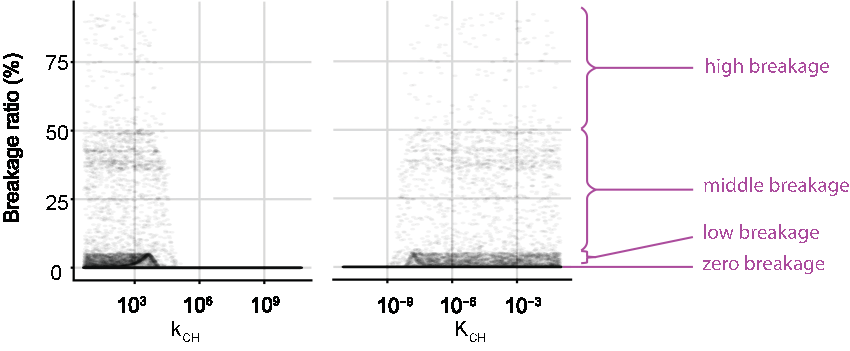
\includegraphics[width=0.95\textwidth, trim={0cm 0cm 0cm 0cm}, clip]{D_chapters/2_ReactionModel/ratesSelection.pdf}
\caption[Breakage ratio modes]%
{Breakage ratio modes observed after  wide sampling around approximate values available in the literature. We optimize the reaction rates using high breakage mode, because it manages to efficiently recruit both myosin and dynein motors.}
\label{figure:BreakageModesRatesSelection}
\end{center}
\end{figure}

Next, we introduced a cost function to evaluate points in this group. It penalizes distance of reaction parameter values from literature values as well as low capsid breakage probability:

\begin{equation}
C = \big| \log_{10} \big( \frac{\%}{\%_{max}} \big) \big| +\\
\sum_{i} \big| \log_{10} \big( \frac{k^i}{k^i_{literature}} \big) \big| +\\
\sum_{i} \big| \log_{10} \big( \frac{K^i}{K^i_{literature}} \big) \big|
\end{equation}

where   is an on rate,   is a dissociation constant, and   is a capsid breakage probability. Because literature parameter values were of the same order of magnitude (approximately   for on rates and   for dissociation constants), we did not introduce extra weight coefficients. We selected the parameter point with minimal value of the cost function as reference point.

To compare the performance of ‘Symmetric’ and ‘Asymmetric’ model variants (Figure 4B, S3B, C, D), we sampled the concentrations (20’000 times), reaction rates (20’000 times), and both together (40’000 times). Concentrations were sampled uniformly between 50\% and 150\%, and log-normally in $\pm$1 orders of magnitude of the value reported in proteomics experiments (proteomicsDB; (Schmidt et al., 2018)). Reaction rates were sampled log-uniformly around the reference value in $\pm$1 orders of magnitude, or log-normally around the reference value with a SD of 0.1.

To examine the influence of each individual parameter on the capsid breakage probability, we simulated the model variants with all but one parameter fixed. The free parameter was sampled log-uniformly 20’000 times for concentrations between 50\% and 150\% of the value reported in proteomics experiments (proteomicsDB; (Schmidt et al., 2018)), and log-uniformly 30’000 times for reaction rate constants around the reference value in $\pm$5 orders of magnitude.

Experimental perturbations, when possible, were translated into model perturbations by changing either reaction rate constants or initial concentrations of reactants (Table S2). We simulated each perturbation 20’000 times similarly to the unperturbed system, with initial concentrations sampled as above and rate constants sampled log-normally around the reference value in $\pm$1 order of magnitude, except for the experiment-specific perturbed parameters or initial conditions, which were sampled in the modified ranges as specified in Table S3.

siRNA for Dynactin2 prevented the binding of dynactin and reduced the amount of available dynein to 1/10 of the norm. Ciliobrevin D, which inhibits the dynein motor activity, stopped the motors from walking, but not from binding; we simulated that case as control, but then assumed zero active dyneins for computing the breakage probability. siRNAs for myosin10 affected the amount of available myosin by reducing it to 1/10 of the norm. siRNAs for myosin9 were not modeled given that experiments showed little effect on the breakage probability. ML-9 and Blebbistatin cases were not simulated as they correspond to zero effective myosins, which, according to the mass-spring model, fails to generate breakage. For the HDAC6 $\Delta$DMC MEF cell line, we assumed an increase of the dissociation constant for HDAC6-dynein binding by a factor of 1000. The HDAC6 KO MEF cell line and siRNA HDAC6 had initial concentrations of HDAC6 reduced to 1/100 and 1/10 of the norm, respectively. The HDAC6 ZnFm (W1116A) MEF cell line had the dissociation constant of HDAC6-Ub binding increased by a factor 1000. We assumed that Cytochalasin D and Nocodazole, which affect actin and tubulin polymerization, reduced the amount of available cytoskeletal scaffolding to 1/10 and 1/100 of the norm, respectively. Importazole is a selective inhibitor of the nuclear transport receptor importin-beta and prevents nuclear import of NLS-containing proteins (Soderholm et al., 2011). MG132 is a proteasome inhibitor, leading to misfolded proteins accumulation in the cell and to a depletion of free cellular ubiquitin chains that are no longer recycled during proteasomal degradation of those proteins; therefore, we assumed a reduction in Ub concentration to 1/10 of the norm.

An alternative and, perhaps, more biologically reasonable approach to model the domain deletion from HDAC6 would be to remove dynein motors and Ub from the simulation entirely. However, doing so in our ODE reaction model leads to the simulation becoming unstable, and ideally requires additional model modifications, making comparisons between the different reaction models difficult. Modifying reaction rates in contrast, allows us to account for random effects of unspecific binding while keeping the model simple and deterministic.

For the M1 binding signal perturbations, we used H1N1 M1 (and its ‘restored’ virus version H3N2 M1 A218T) as a control, and H2N2 M1 (and its ‘restored’ virus version H1N1 M1 T218A) as a perturbation that increases the HDAC6-capsid dissociation constant by a multiplication factor. We used the average M1 binding signal for the H1N1 M1 T218 mutant and H3N2 WT (Figure 6E), and fitted a corresponding value of binding to capsid breakage in our individual parameter perturbation experiments (Figure 4C, D). The final multiplication factor values were 14.6 for the ‘Asymmetric’ and 23.7 for the ‘Symmetric’ model variant.

For the virus infectivity perturbations, we considered pH1N1 ko/ki WT to be a control, H3N2 ko/ki WT, corresponding to M1-HDAC6 binding dissociation constant being increased by the multiplication factor above, pH1N1 ko/ki ZnF mutant to have an increased ofHDAC6-Ub dissociation constant by a factor of 1000, and H3N2 ko/ki ZnF mutant as both.

